%!TEX root = stokes_paper.tex

\section{Examples \label{sec:results}}
In this section, the lightning Stokes solver is tested on various sample problems found in the literature. We present contour plots for the stream function $\psi$ superimposed on a color plot of the velocity magnitude. We use black contours for the first Moffatt eddy, and subsequent ones are highlighted in yellow. The convergence plots indicate root-exponential convergence as expected. We also provide a close-up of the eddies.

\begin{figure}[H]
	\centering
	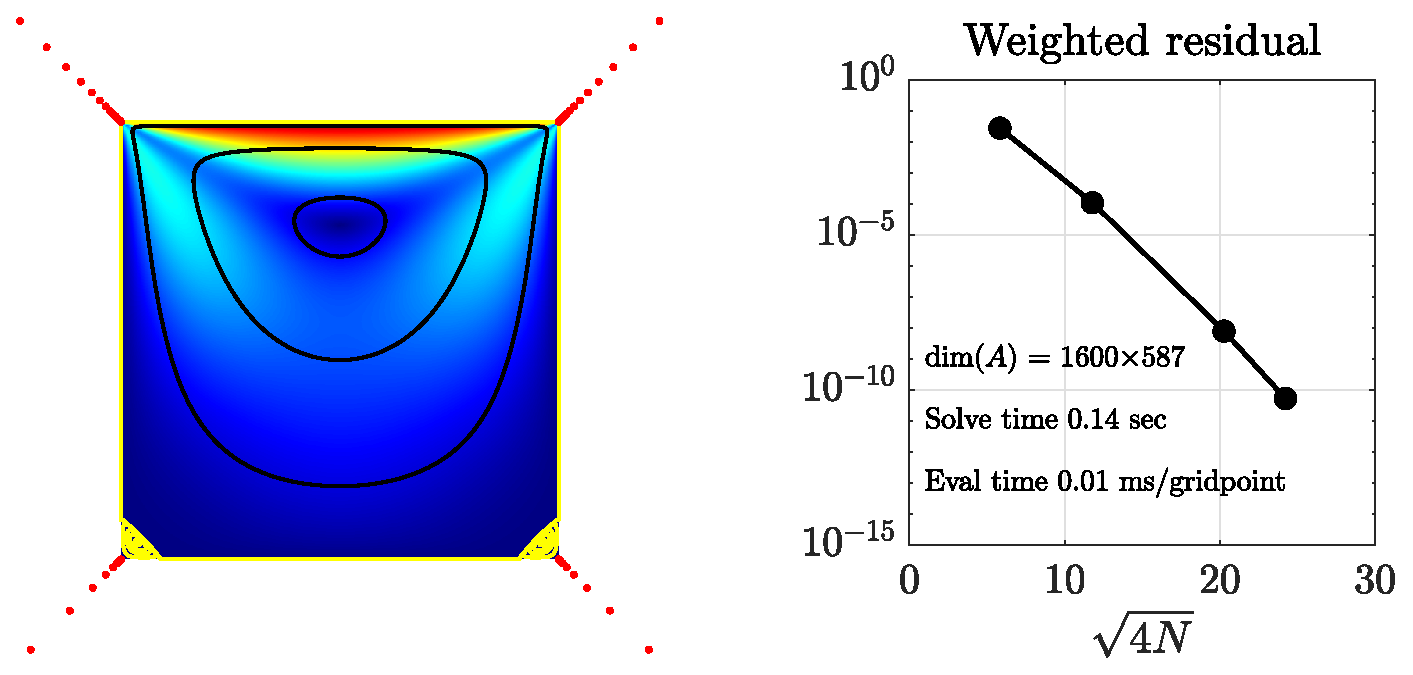
\includegraphics[width=\linewidth]{Figures/ldc}
	
	\vspace{2em}
	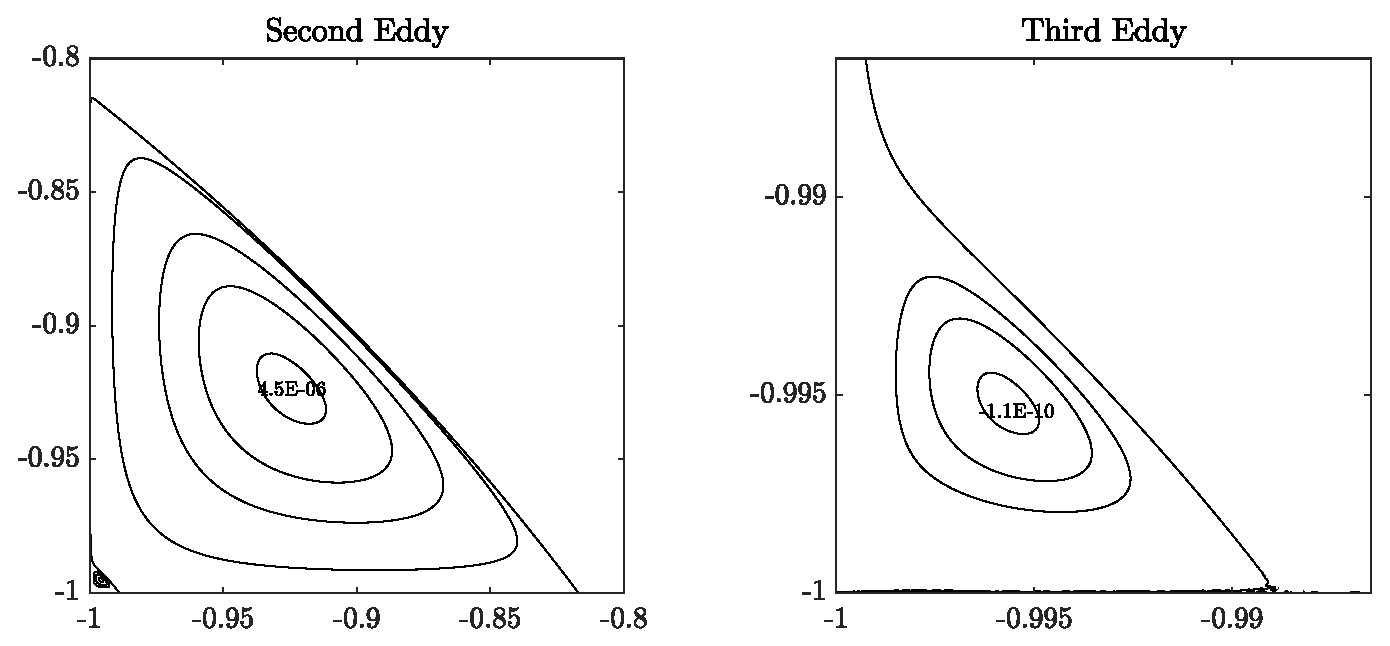
\includegraphics[width=\linewidth]{Figures/ldc_eddy}
	\label{fig:ldc}
	\caption{Stokes flow inside a square lid-driven cavity. In this example, a fluid is enclosed inside a cavity, whose lid moves from left to right with unit speed, and no-slip boundary conditions are imposed at the other 2 surfaces.}
\end{figure} 

\begin{figure}[H]
	\centering
	\begin{minipage}{0.45\linewidth}
		\centering
		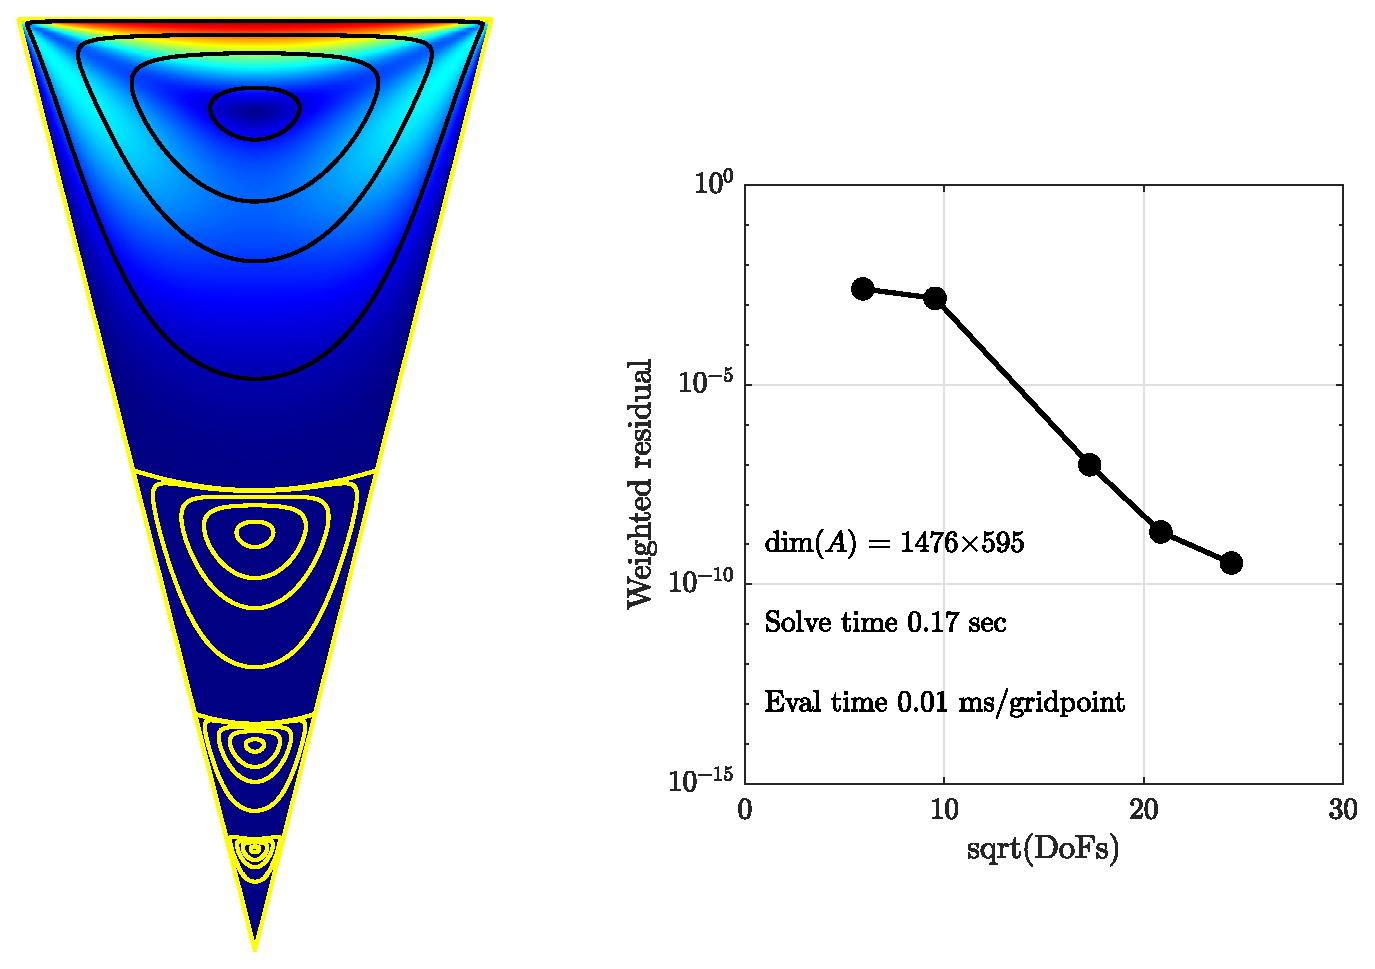
\includegraphics[width=\linewidth]{Figures/wedge}
	\end{minipage}
	\hfill
	\begin{minipage}{0.45\linewidth}
		\centering
		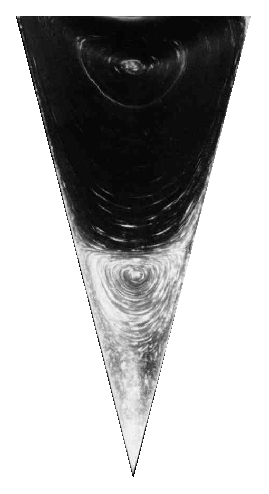
\includegraphics[width=0.6\linewidth]{Figures/wedge_exp}
	\end{minipage}

	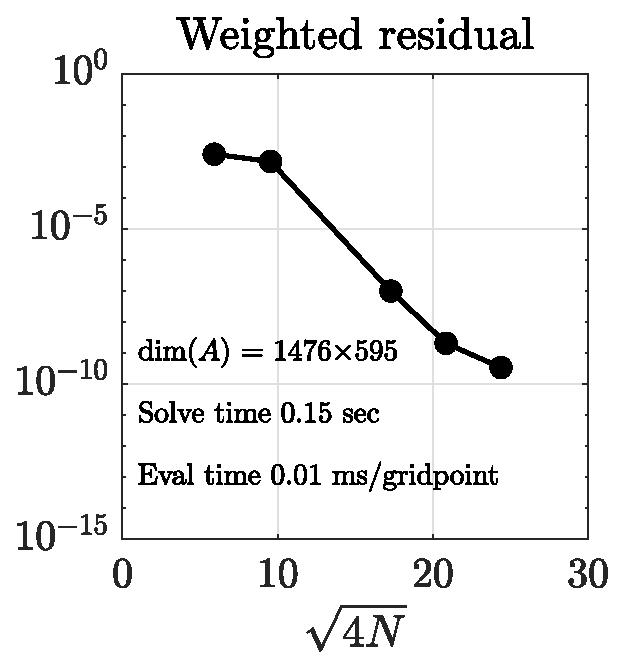
\includegraphics[width=0.5\linewidth]{Figures/wedge_conv}
	
	
	\label{fig:wedge}
	\caption{Stokes flow inside a wedge of total angle $28.5^\circ$. The top lid moves from left to right with unit speed and no-slip boundary conditions are imposed at the other 2 surfaces. For comparison, the first two eddies have been observed experimentally by Taneda in \cite[Fig.~19]{taneda79}, also included in \cite[Fig.~10]{vandyke82}, for a very similar setup driven by a rotating cylinder with $\text{Re}=1.7\times10^{-1}$.}
\end{figure} 

\begin{figure}[H]
	\centering
	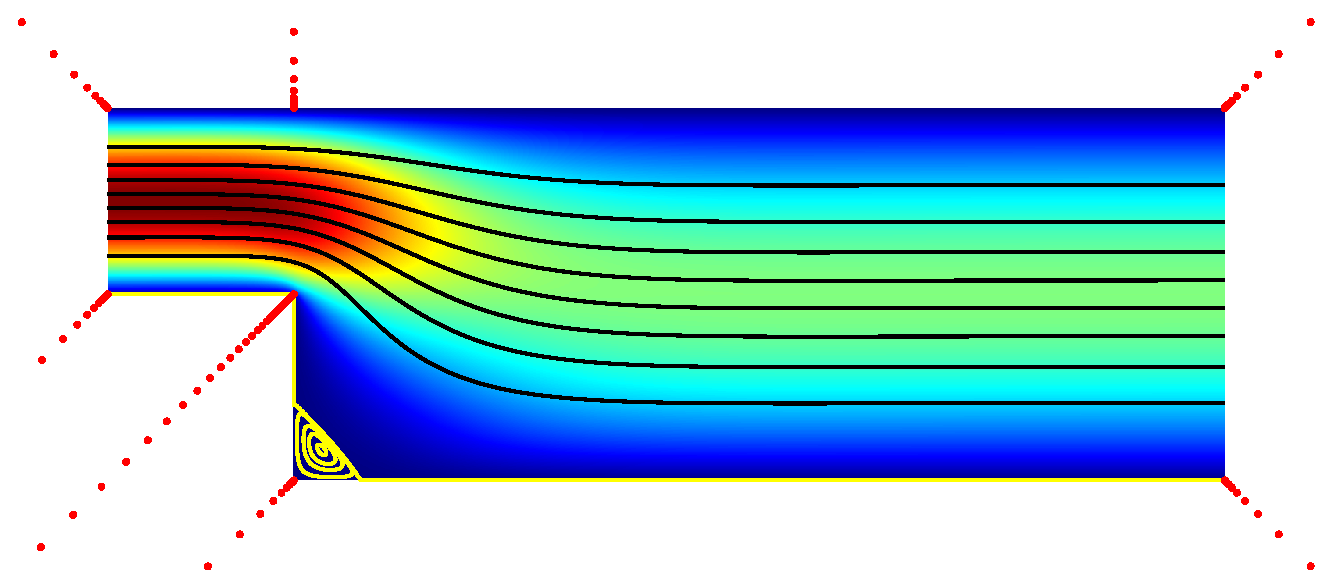
\includegraphics[width=\linewidth]{Figures/step}
	
	\vspace{2em}
	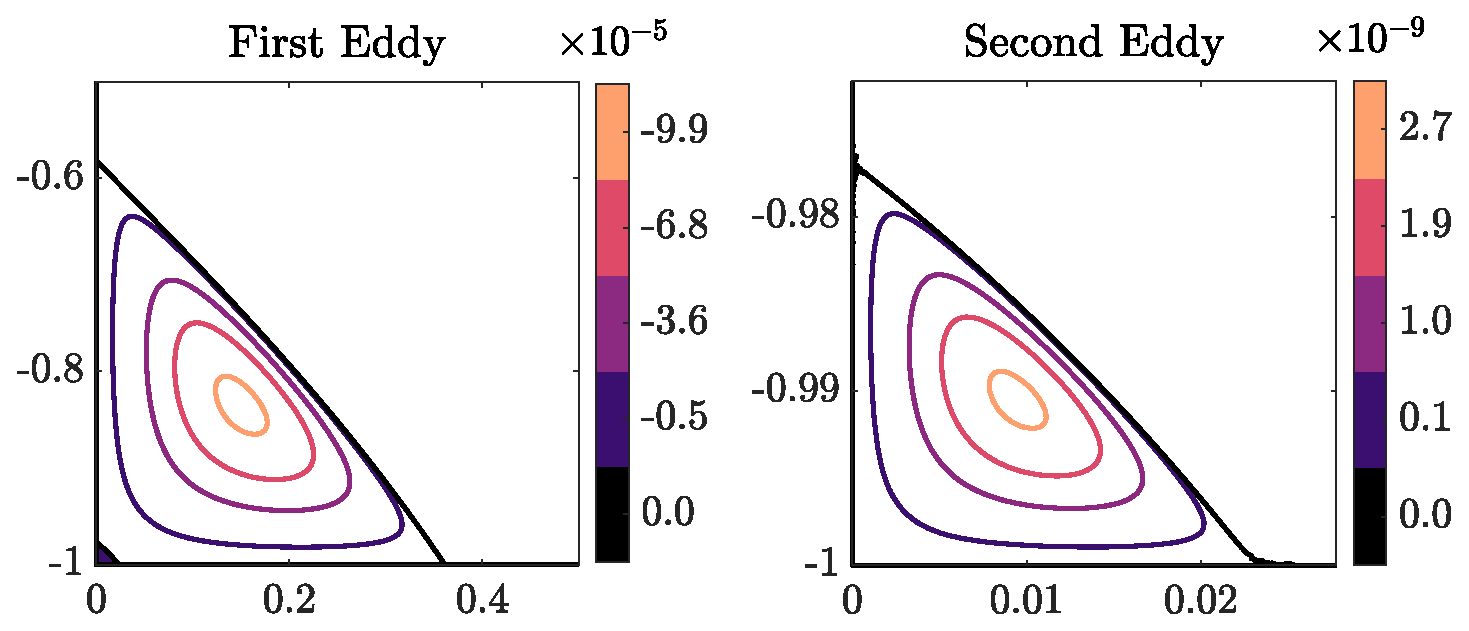
\includegraphics[width=\linewidth]{Figures/step_eddy}
	
	\vspace{2em}
	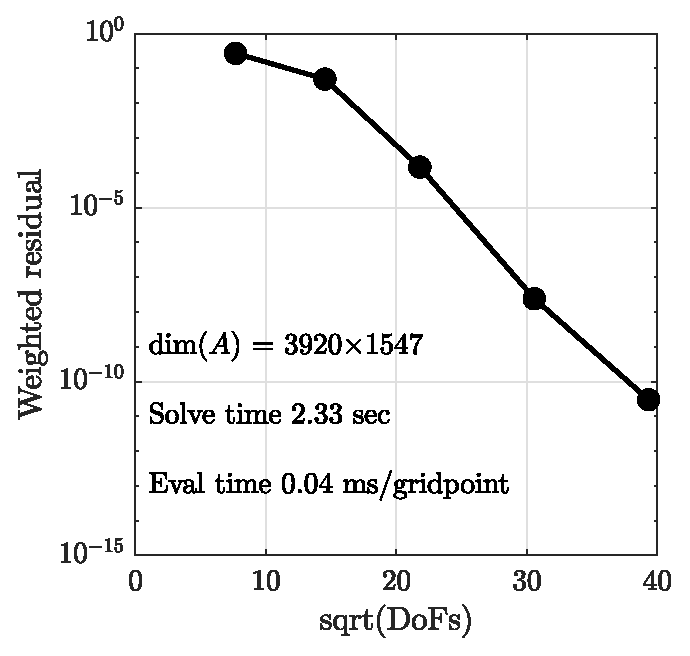
\includegraphics[width=0.5\linewidth]{Figures/step_conv}
	
	\label{fig:step}
	\caption{Stokes flow over a step. A parabolic profile is prescribed at the inflow and at the	outflow, a no-slip condition is imposed on the rest of the walls. At the re-entrant corner the pressure and the derivatives of the velocity become unbounded.}
\end{figure} 

\section{Unbounded domains \label{sec:unbounded}}


\begin{figure}[H]
	\centering
	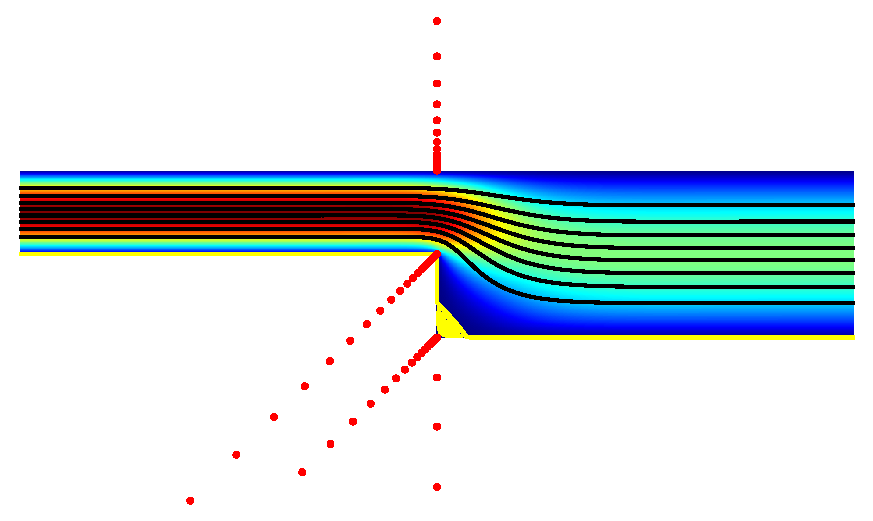
\includegraphics[width=\linewidth]{Figures/chan}
	
	\vspace{2em}
	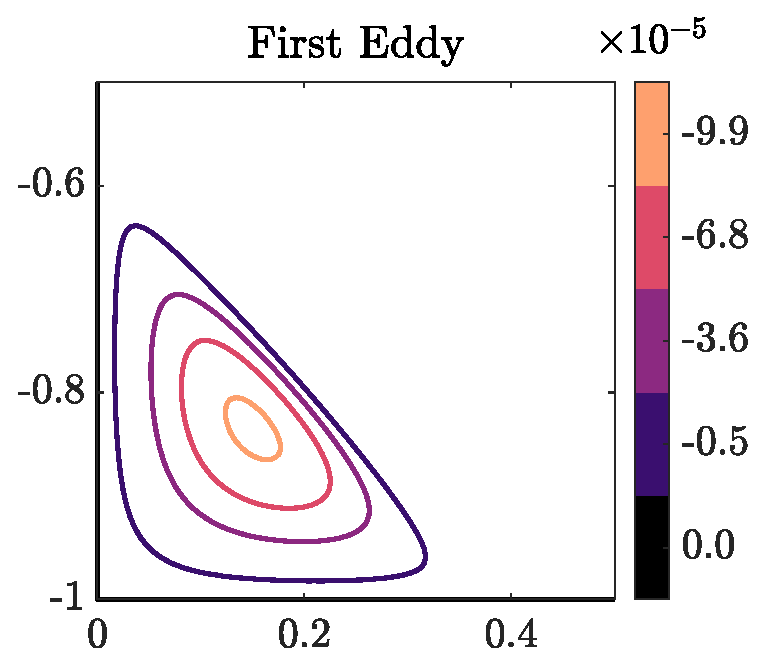
\includegraphics[width=0.45\linewidth]{Figures/chan_eddy}
	\hfill
	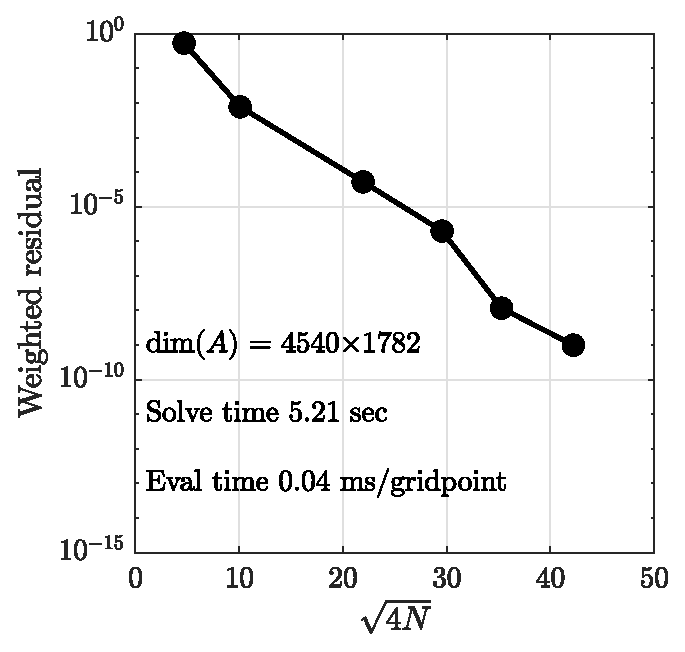
\includegraphics[width=0.45\linewidth]{Figures/chan_conv}
	
	\label{fig:chan}
	\caption{Stokes flow inside an infinitely long pipe with an expansion.}
\end{figure} 

\section{Multiply connected domains \label{sec:multiply}}


